\begin{figure}[ht!]
    \centering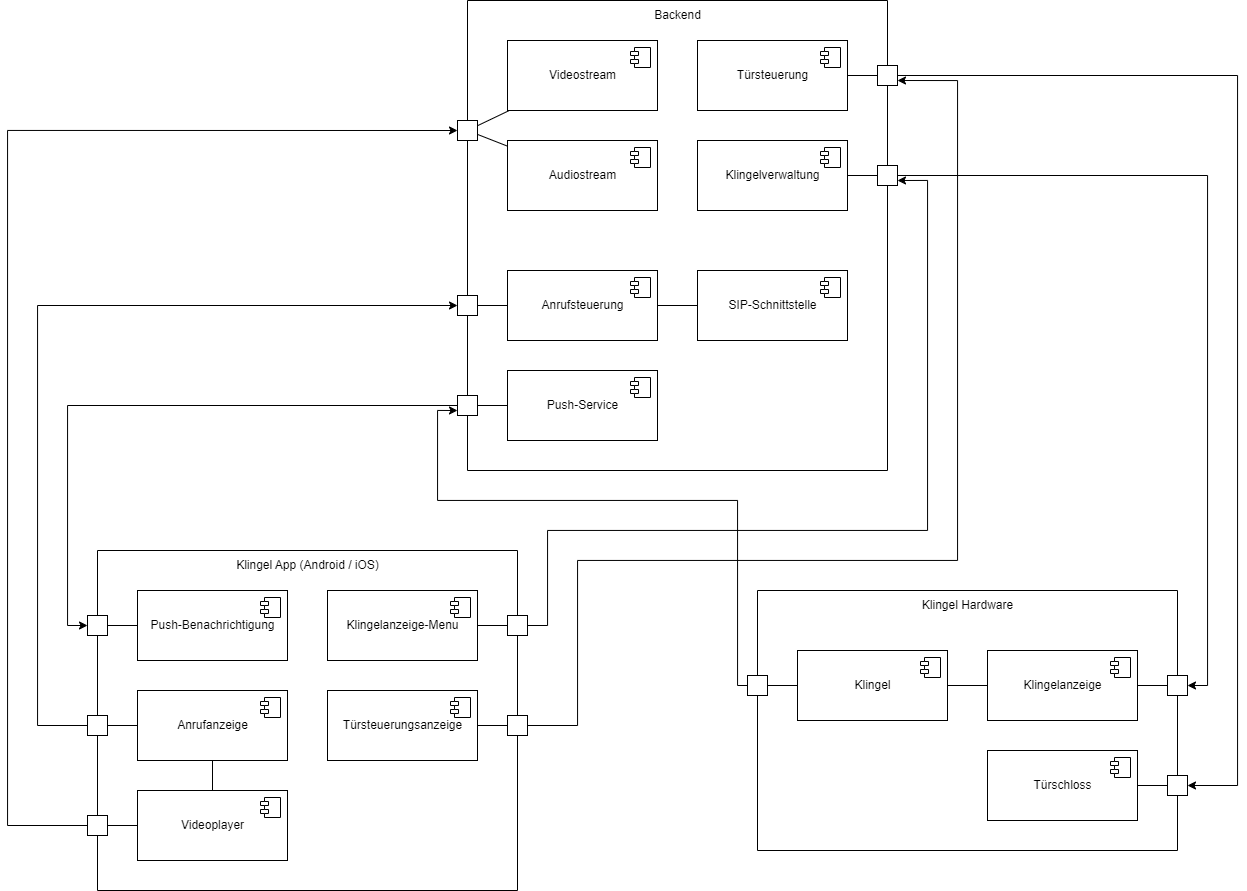
\includegraphics[width=\paperwidth-2in]{../assets/img/Komponentendiagramm}

    \caption{Komponenten von App, Hardware und Backend}
    \label{fig:komponentendiagramm}
\end{figure}
In Abbildung~\ref{fig:komponentendiagramm} ist das Komponentendiagramm dargestellt.
Dabei besteht die Klingel Hardware aus der Klingel selbst, die den Push-Service im Backend aktivieren muss 
und aus der Klingelanzeige, auf der nach Wunsch ein Name oder nur die Wohnungsnummer angezeit werden kann.
Außerdem ist die Türschloss-Komponente dafür da, die Tür auf- und zuzuschließen.

Das Backend wird um den Push-Service erweitert, der eine Push-Benachrichtigung senden kann.
Außerdem die Anrufsteuerung zum Steuern der Anrufe nach dem SIP-Standard.
Desweiteren gibt es im Backend die Audio- und Videostream Komponenten, die für die Anrufe selbst wichtig sind.
Diese können Audio und Video an die Klingel-App übertragen.
Die Türsteuerung ist dafür da das Türschloss zu kontrollieren und die Klingelverwaltung kann die Klingelanzeige in der Klingel-Hardware steuern.

Im dritten Subsystem, die Klingel-App, gibt es zum einen die Komponente der Push-Benachrichtigung.
Außerdem das Klingelanzeige-Menu, welche von der Klingelverwaltung eine Übersicht aller Klingeln anzeigen kann.
Die Türsteuerungsanzeige ist wesentlich die Visualisierung der Türsteuerung.
Zuletzt gibt es noch die Anrufanzeige in Verbindung mit dem Videoplayer, die jeweils mit Video- und Audiostream und der Anrufsteuerung im Backend komunizieren.
So kann der Benutzer den Anruf über die Visualisierung steuern und gegebenfalls das übertragene Video sehen.